% Dependency graph of the Dubroff--Fox--Xu note (drawn by hand).
\begin{tikzpicture}[x=1cm,y=1cm,
  box/.style={draw=black!60,rounded corners=2pt,align=center,font=\scriptsize,inner sep=3pt,fill=white},
  cited/.style={box,fill=black!6,dashed},
  arr/.style={->,>=stealth,black!60}]
\node[box,fill=orange!15] (T) at (0,0) {Theorem 1\\ $a_n\ge(\sqrt{2/\pi}-o(1))\,2^n/\sqrt n$};
\node[box] (P1) at (-3.2,1.6) {first proof\\ (two cases)};
\node[box] (P2) at (3.2,1.6) {second proof\\ $a_n\ge\binom n{\lfloor n/2\rfloor}$};
\node[cited] (M) at (-5.2,3.3) {Moser:\\ $\sum a_i^2\ge\frac{4^n-1}3$};
\node[cited] (BE) at (-3.0,3.3) {Berry--Esseen\\ (non-identical)};
\node[box] (C) at (-0.9,3.3) {window count\\ $P(|X|\le\ell)\le\frac{\ell+1}{2^n}$};
\node[cited] (H) at (2.0,3.3) {Harper's vertex\\ isoperimetry};
\node[box] (D) at (4.6,3.3) {signed differences\\ $|a\cdot(\epsilon-\eta)|\ge1$};
\node[box,fill=red!10] (L) at (2.0,4.9) {shortcut: Lubell's chains?\\ fails (size matters)};
\draw[arr] (M)--(P1); \draw[arr] (BE)--(P1); \draw[arr] (C)--(P1);
\draw[arr] (H)--(P2); \draw[arr] (D)--(P2);
\draw[arr] (P1)--(T); \draw[arr] (P2)--(T);
\draw[arr,red!60!black,dashed] (L)--node[midway,right,font=\tiny]{$\times$}(H);
\node[font=\tiny,black!60] at (-5.2,4.05) {(Chapter~1)};
\node[font=\tiny,black!60] at (-3.0,4.05) {(Tome~10, adapted)};
\end{tikzpicture}
